\documentclass{standalone}
\usepackage{tikz}

\begin{document}

% First Image: Rectangle with Circle and Unit Vectors
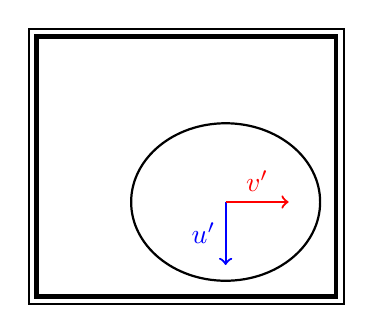
\begin{tikzpicture}
    % Draw rectangle
    \draw[thick] (0, 0) rectangle (4, 3.5);
    \draw[ultra thick] (0.1, 0.1) rectangle (3.9, 3.4);

    % Draw ellipse (stretched in v direction and shifted down-right)
    \draw[thick, rotate=0] (2.5, 1.3) ellipse (1.2 and 1); % Stretched in y-direction

    % Draw unit vectors
    \draw[->, thick, blue] (2.5, 1.3) -- (2.5, 0.5) node[midway, left] {$u'$}; % Down
    \draw[->, thick, red] (2.5, 1.3) -- (3.3, 1.3) node[midway, above] {$v'$}; % Right
\end{tikzpicture}

\end{document}